\documentclass[a4paper, 12pt]{article}
\usepackage[utf8]{inputenc}
\usepackage{enumitem}
\usepackage{graphicx}
\usepackage{float}
\usepackage{polski}
\usepackage{subfig}
\usepackage{hyperref}
\usepackage{mathtools}

\title{Multimedia and Computer Visualization}
\author{Rafał Grądkowski, Bartosz Gardziejewski, Paweł Zaborowski, Łukasz Obrębski}
\date{15th January 2020}

\begin{document}

\begin{titlepage}
    \makeatletter
    \vspace{1cm}
    \begin{center}
        
\includegraphics[width=0.75\textwidth]{PWr-logo_ang.png} \par
        \vspace{0.2cm}
        \Large Faculty Of Electronics \par
        \vspace{1.25cm}
        {    
            \bfseries
            Computer Science \\
            \vspace{0.25cm}
    	    \normalsize Internet Engineering \par
    	    \vspace{2cm}
    	    \Huge \@title \\
    	}
    	\vspace{0.5cm}
        \large Digital Watermarking
    \end{center}
    \null
    \vfill
    \begin{flushright}
        Authors: \\
        Rafał Grądkowski \\
        Bartosz Gardziejewski \\
        Paweł Zaborowski \\
        Łukasz Obrębski
    \end{flushright}
    \vspace{0.5cm}
    \begin{flushleft}
        Lecturer: dr inż. Marek Woda \break
        Group: E05-17b \par
    \end{flushleft}
\end{titlepage}

\newpage
\title{Digital Watermarking}

	
\newpage
\tableofcontents

\newpage

\section{Subject}

The project's aim is to implement and compare two digital watermarking methods when applied to images. Chosen technologies are Least Significant Bit [LSB] Technique and Patchwork Algorithm.
Analysis will be focused on main areas of watermarking which are: transformation, distortion, compression...
\\ \\
//TODO: dopisac jakie jeszcze. 

\section{State of the art}

Digital watermarking in general is a kind of marker embedded in a noise-tolerant signal. The most popular kinds of the signals which allow watermarking are images, videos and audio signals. Digital watermarking techniques are typically used for identifying ownership and mark copyrights. Most recognizable form of digital watermarking in images is a simple overlay of a text or logo image over the original image. An example of such watermark can be seen below:

\begin{center}
    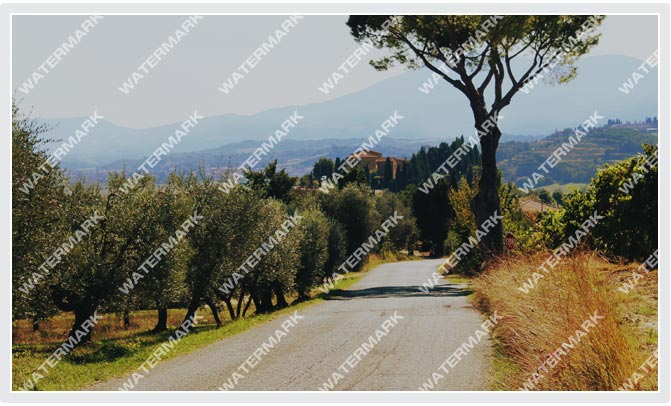
\includegraphics[width=1\textwidth]{ex.png} \par
\end{center}

However, in professional applications, digital watermarks should be perceptible under certain conditions only, e.g. after using some specific algorithm. If the carrier signal is distorted by a digital watermark in such a way that it becomes easily noticable or the size of the carrier signal is changed, it could be considered not effective (depending on its purpose. \par

There are currently three types of digital watermarking methods:

\begin{enumerate}
	\item Spatial domain techniques - directly add the watermark to pixel values - exploit Human Visual System for hiding the data
	\item Transformed domain techniques - add the watermark to the coefficients of a full-frame transform (DFT, DCT, Mellin, Radon, Fresnell)
	\item Hybrid techniques
\end{enumerate}

\section{Project's scope}

A concise project's description was done in the following subchapters, consisting of information about project's goal, requirements and implemented features.

\subsection{Goal of the project}
The main goal of the project is to prepare simple application with both of the algorithms implemented. Our tasks were focused on proper algorithm implementation rather than on user interface. We were trying to implement both algorithms properly and to compare parameters between them. Also our aim was to compare how do they work in practice.

\subsection{Requirements}

The user need to have possibility to encode their picture by watermark, optionally, chosen by them. The user need to have possibility to choose which algorithm they would like to use.

\subsection{Features}

Application is Command Line Interface based. Firstly it allows user to choose between encoding picture, or with usage of patchwork, decoding, shown on the figure a). After picking encoding we have two algorithms to choose (figure b)).

\begin{figure}[!h]%
	\centering
	\subfloat[figure a)]{{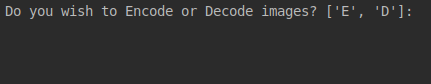
\includegraphics[width=5cm]{ui_intro.png} }}%
	\qquad
	\subfloat[figure b) ]{{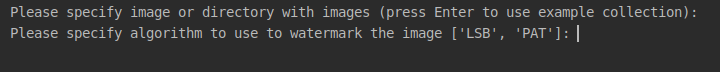
\includegraphics[width=5cm]{ui_alg_choose.png}}}%
	\label{}%
\end{figure}

\subsubsection{Encoding}

\begin{itemize}
	\item LSB
		Application requests either for picture to be watermarked and the one to be used as watermark. 
		
		 \begin{center}
			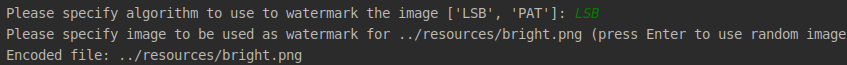
\includegraphics[width=1\textwidth]{ui_lsb.png}
		\end{center}
	
	\item Patchwork
	
		In opposition to previous option there application needs to provide encoding key.
		 \begin{center}
			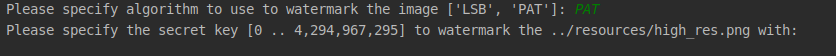
\includegraphics[width=1\textwidth]{ui_pw_choose.png}
		\end{center}
		
\end{itemize} 

\subsubsection{Decoding}

	 \begin{center}
		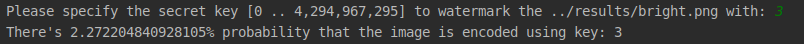
\includegraphics[width=1\textwidth]{ui-pw-decode.png}
	\end{center}
	
	

\section{Techniques and Technologies}
	
	\subsection{Tools}
	
	\begin{itemize}
		\item Python 3.7 with packages:
		\begin{enumerate}
            \item NumPy
            \item scikit-image
        \end{enumerate}
		\item Algorithms: \begin{enumerate}
			\item LSB – Least Significant Bit
			\item Patchwork techniqe
		\end{enumerate}
	\end{itemize}
	
\subsection{Communication between team members}
Communication of team members took place remotely using Trello (an internet
application for project management) and Facebook Messenger (messenger on a social
networking site). After the division of tasks through Trello, each member could take on	a specific task and present the progress of the work and the final effects of the project stages on an ongoing basis. Important point of communication were team meetings, where we could discuss problems related to the project implementation and solve difficult tasks more efficient. The source code of the application has been managed remotely using the GitHub repository.
	
\section{Milestone and project plan}

	\subsection{Team members}
	
	\begin{itemize}
		\item Bartosz Gardziejewski
		\item Rafał Gradkowski
		\item Łukasz Obrebski
		\item Paweł Zaborowski
	\end{itemize}

	\subsection{Project plan}
	
	Out team have splitted into topic groups:
	
	\begin{enumerate}
		\item LSB implementation
		\item Patchwork implementation
		\item Documentation work
	\end{enumerate}
	

	\subsection{Gantt Chart}
	
	\begin{itemize}
	

	\item 11.10.19 – Setup of Trello \& GitHub
	\item 17.10.19 – Project Kick OFF (first presentation)
	\item 14.11.19 – Literature analysis, working Python environment, beginnings of a documentation
	\item 28.11.19 – Implementation of embedding digital watermark in images using both algorithms
	\item 12.12.19 – Implementation of decoding digital watermark in images using both algorithms
	\item 09.01.20 – Juxtaposition and comparison of results
	\item 16.01.20 – Project closure (Final presentation, project demo, documentation)
	\end{itemize}
	
\section{Results}

	\subsection{LSB}

	    \subsubsection{Implementation}
    	In our program the LSB algorithm is going through the image colour by colour and pixel by pixel and checks the most significant bit of the watermark pixel, if it is 1 then it sets 1 in lest significant bit of the pixel in image, if it is 0 then it is set to 0. If the water mark is smaller then image it is looped.

    	\subsubsection{Testing}
    	We performed test using our LSB algorithm on two pictures. The results was as follows.
    	Firs picture was python logo with resolution 225x225 it take approximately 1 second to watermark that image and the second was photo with resolution 393x206 it take approximately 1.5 second:

	\begin{figure}[!h]%
		\centering
		\subfloat[]{{
\includegraphics[width=5cm]{python_lsb/python_original.png} }}%
		\qquad
		\subfloat[]{{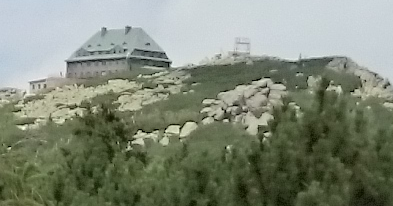
\includegraphics[width=5cm]{photo_lsb/Photo_original.png}}}%
		\label{}%
	\end{figure}	

     
    	
        As watermark we used small python logo with resolution 64x64 and color inversion:

        \begin{center}
            
\includegraphics[scale=1.5]{watermark.png}
        \end{center}
    	
        Watermarked image and the water mark extracted from it looked as expected as on figure: %\autoref{fig:python_logo}:
        
        \begin{figure}[!h]%
        	\centering
        	\subfloat[]{{
\includegraphics[width=5cm]{python_lsb/watermarked_python.png} }}%
        	\qquad
        	\subfloat[]{{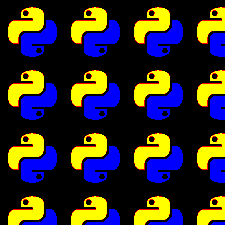
\includegraphics[width=5cm]{python_lsb/watermark_photo.png}}}%
        	\label{fig:python_logo}%
        \end{figure}


        \begin{figure}[!h]%
			\centering
			\subfloat[]{{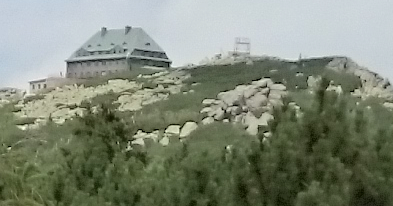
\includegraphics[width=5cm]{photo_lsb/watermarked_photo.png} }}%
			\qquad
			\subfloat[]{{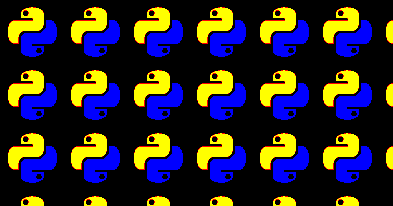
\includegraphics[width=5cm]{photo_lsb/watermark_photo.png}}}%
			\label{fig:python_logo2}%
		\end{figure}

        
    	Next step was to transform the watermarked image and check if watermark is extractable from it. To perform transformation we used program GIMP2.0. First we try rotating image by 45 degrees, figure %\autoref{fig:45}:

        \begin{figure}[h]%
			\centering
			\subfloat[]{{
\includegraphics[width=5cm]{python_lsb/watermark_python_rot45.png} }}%
			\qquad
			\subfloat[]{{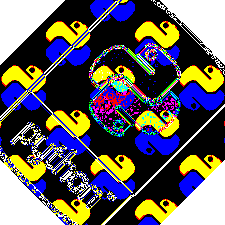
\includegraphics[width=5cm]{python_lsb/watermark_watermark_python_rot45.png}}}%
			\label{fig:45}%
		\end{figure}

		\begin{figure}[h]%
			\centering
			\subfloat[]{{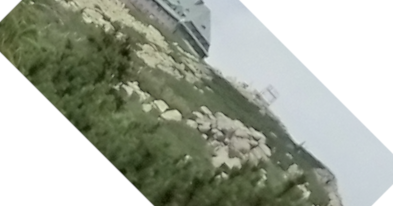
\includegraphics[width=5cm]{photo_lsb/watermarked_photo_rot45.png} }}%
			\qquad
			\subfloat[]{{
\includegraphics[width=5cm]{photo_lsb/watermark_watermarked_photo_rot45.png}}}%
			\label{}%
		\end{figure}
	
	\newpage

    	Expected outcome of the rotation would be rotated wtermark, but in this case we could see distortion around edges in \textit{python} logo and absolutely unreadable watermark in \textit{photo}. It turns out that some programs have more complex rotation algorithm to maker rotated image look better. Next we try color inversion:
    	
 		\begin{figure}[!h]%
    		\centering
    		\subfloat[]{{
\includegraphics[width=5cm]{python_lsb/watermark_python_invert.png} }}%
    		\qquad
    		\subfloat[]{{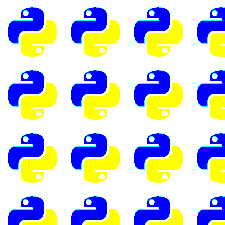
\includegraphics[width=5cm]{python_lsb/watermark_watermark_python_inver.png}}}%
    		\label{}%
    	\end{figure}


    	In this case as expected watermark was color inverted only. Next we try manipulate with color, and change contrast:

 		\begin{figure}[!h]%
			\centering
			\subfloat[]{{
\includegraphics[width=5cm]{python_lsb/watermark_python_colMod.png} }}%
			\qquad
			\subfloat[]{{
\includegraphics[width=5cm]{python_lsb/watermark_watermark_python_colMod.png}}}%
			\label{}%
		\end{figure}


    	It Turns out that even slightly changed contrast makes watermark almost unreadable. Last transformation was more advanced one, performed on \textit{photo}.

    	Noise reduction:

 		\begin{figure}[!h]%
			\centering
			\subfloat[]{{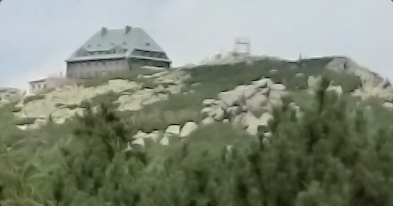
\includegraphics[width=5cm]{photo_lsb/watermarked_photo_reduction.png} }}%
			\qquad
			\subfloat[]{{
\includegraphics[width=5cm]{photo_lsb/watermark_watermarked_photo_reduction.png}}}%
			\label{}%
		\end{figure}

		Gaussian blur:

 		\begin{figure}[!h]%
			\centering
			\subfloat[]{{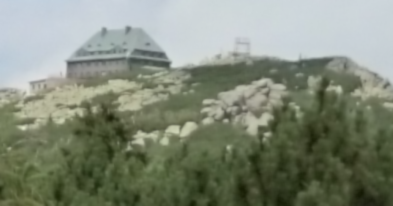
\includegraphics[width=5cm]{photo_lsb/watermarked_photo_gaus.png} }}%
			\qquad
			\subfloat[]{{
\includegraphics[width=5cm]{photo_lsb/watermark_watermarked_photo_gaus.png}}}%
			\label{}%
		\end{figure}


   	They both almost completely destroyed watermark.

	\subsection{Patchwork algorithm}
	
	\subsubsection{Implementation}
	
	Patchwork algorithm variation used in the project, was implemented as follows:
	
	\begin{itemize}
	 \item Convert image color model to YUV.
	 \item Randomly (based on certain key) select N pairs of pixels.
	 \item Increase first pixel's Y channel value by a constant value $\delta$. Decrease second pixel's Y channel value analogically.
	 \item Convert image color model back to original.
	\end{itemize}
	
	Now, to detect such watermark, key must be known to obtain the same pairs of pixels during image decoding. Then, pixels pairs are 'visited' in the same order, to calculate control sum as follows:
	
	\begin{equation}
	 \sum_{i=0}^{N} A_i - B_i \\
	\end{equation}

    where $A_i$ and $B_i$ are first and second pixel's Y channel values respectively. \\
    
    It is expected that for unmodified image control sum value will be close to 0, as the number of times $A_i$ is greater than $B_i$ should be offset by the number of times the reverse is true.
    
    Unfortunately, this assumption is not always true, which is the main disadvantage of currect implementation, as can be seen in the next section.
	
	\subsubsection{Testing}



\section{Conclusions}

	\subsection{LSB}

	LSB is fairly simple and quite fast algorithm, unfortunately it is not very robust - simple transformation can make it "disappear". We could use for example not the least significant bit but middle one that should increase robustness, although it makes watermark much more visible:



	 \begin{center}
		
\includegraphics[scale=0.5]{python_lsb/watermarked_python_4bit.png}
	\end{center}

	LSB pros and cons:
	\begin{itemize}

		\item Resistance to geometric transformations, like cropping, stretching or rotating, in condition that the operation is not using more sophisticated algorithm
		\item High capacity of watermark
		\item fast and easy to implement
		\item Can be easily destroyed by distortions or gamma changes




	\end{itemize}

	\subsection{Patchwork}
	
	Patchwork pros and cons

	\begin{itemize}
		\item Resistance to cropping and to gamma and tone scale corrections
		\item The detector doesn’t require the original cover image to determine whether the image has been watermarked.
		\item Can be destroyed by any affine transformation, like translation, rotation or scaling
	\end{itemize}

\end{document}
